% This is samplepaper.tex, a sample chapter demonstrating the
% LLNCS macro package for Springer Computer Science proceedings;
% Version 2.20 of 2017/10/04
%
\documentclass[runningheads]{llncs}
%
\usepackage{graphicx}
\usepackage{wrapfig}
%\usepackage{amsthm}
\usepackage{amssymb}
\usepackage{mathtools}
\DeclarePairedDelimiter\abs{\lvert}{\rvert}
\DeclarePairedDelimiter\norm{\lVert}{\rVert}
\DeclarePairedDelimiter\inner{\langle}{\rangle}
\def\P{\mathcal{P}}
\DeclareMathOperator*{\argmin}{argmin}

\usepackage{algorithm}
\usepackage{algorithmic}
\makeatletter
\newcommand{\algorithmicfunction}{\textbf{function}}
\newcommand{\algorithmicendfunction}{\algorithmicend\ \algorithmicfunction}
\newenvironment{ALC@func}{\begin{ALC@g}}{\end{ALC@g}}
\newcommand{\FUNCTION}[2][default]{\ALC@it\algorithmicfunction\ #2\ %
\textbf{:}%
\ALC@com{#1}\begin{ALC@func}}
\ifthenelse{\boolean{ALC@noend}}{
    \newcommand{\ENDFUNCTION}{\end{ALC@func}}
  }{
    \newcommand{\ENDFUNCTION}{\end{ALC@func}\ALC@it\algorithmicendfunction}
  }
\makeatother

% Used for displaying a sample figure. If possible, figure files should
% be included in EPS format.
%
% If you use the hyperref package, please uncomment the following line
% to display URLs in blue roman font according to Springer's eBook style:
% \renewcommand\UrlFont{\color{blue}\rmfamily}

\begin{document}
%
\title{Info-Detection: An Information-Theoretic Approach to Detect Outlier}
%
%\titlerunning{Abbreviated paper title}
% If the paper title is too long for the running head, you can set
% an abbreviated paper title here
%
\author{Feng Zhao\inst{1} \and
Fei Ma\inst{2} \and
Yang Li\inst{2} \and
Shao-Lun Huang \inst{2} \and
Lin Zhang\inst{1,2}}
%
\authorrunning{Feng Zhao et al.}
% First names are abbreviated in the running head.
% If there are more than two authors, 'et al.' is used.
%
\institute{Department of Electronic Engineering, Tsinghua University \and
Tsinghua-Berkeley Shenzhen Institute, Tsinghua University \\
\email{zhaof17@mails.tsinghua.edu.cn, mf17@mails.tsinghua.edu.cn, yangli@sz.tsinghua.edu.cn, shaolun.huang@sz.tsinghua.edu.cn, linzhang@tsinghua.edu.cn}
}
%
\maketitle              % typeset the header of the contribution
%
\begin{abstract}
Outlier detection is one of major task in unsupervised learning. We propose a cluster analysis based outlier detection method called Info-Detection. Info-Detection determines the number of outliers automatically and captures the global property of the provided data. To implement Info-Detection and overcome the global computational complexity, we use principal sequence of partition, which we improve one order of magnitude faster than the original version. Experiments show that compared with other outlier detection methods, Info-Detection achieves better accuracy with an affordable time overhead.

\keywords{Outlier Detection \and Clustering \and Principal Sequence of Partition.}
\end{abstract}
%
%
%
\section{Introduction}
Outlier detection is an important task in data mining. It is the identification of abnormal data (called outliers) which differs from the majority of the data (called inliers) \cite{grubbs1969procedures}. It has applications in fraud detection, loan application processing, activity monitoring etc.\cite{Hodge2004}. Many existing detection algorithms give an outlier score to each data point and the outliers are chosen as those points with highest scores. These methods need to know the number of outliers $n$ in advance but for real-world task, we do not know how many outliers there are and mismatched $n$ produces no good result. Also, besides distance metric, many outlier detection methods have other hyper parameters to tune, which depends heavily on dataset. 

To overcome these problems, we propose Info-Detection, which do not require $n$ in advance and is determined totally by the similarity metric used.  
Info-Detection is a cluster analysis based method. In this domain, some authors use hierarchical density-based method to do outlier detection, which is closed related with DBSCAN and single linkage clustering \cite{Campello}. The density threshold matters. Info-Detection comes from info-clustering, which is a global clustering method \cite{RN1} and need not to choose the hierarchical threshold for detection task. Info-clustering has solid theoretical foundations from information theory and can produce hierarchical tree for the random variables to be clustered. It can also be used to cluster data. In such case, the clustering result is the same as minimum cost clustering with $\beta = 1$ in \cite{RN7}. In this paper, we combine info-clustering with graph theory and propose Info-Detection, which captures the global property of the dataset.  

Though info-clustering has good theoretical properties, it has high time complexity to compute, which limited its application. In this paper, we improve the implementation of info-clustering, which is one order of magnitude faster than the original one. We also propose a prediction scheme which can predict new observations in linear time complexity. To demonstrate our method, we prepare some datasets and test Info-Detection and other methods on them. Empirical comparison shows that Info-Detection gives best result on these datasets and is suitable for different kinds of data. 

The notational convention of this paper is as follows: Let $x_i$ represents the feature vector for the $i$-th data point in the dataset. The directed graph is denoted by $G(V, E)$. Node index set $V=\{1, 2,\dots, \abs{V}\}$. Node set $Z_V=\{Z_i | i \in V\}$. Edge set $E$ is the collection of tuple $(i,j)$. For $B\subseteq V$, edge subset $E(B) = \{(i,j)| i, j \in B,(i,j)\in E\}$ is the edge set restricted on $B$. Each edge is associated with a non-negative weight $w_{ij}$, which is computed from $x_i$ and $x_j$ with a given affinity metric. $\P$ is a partition of $V$. That is, $P=\{C_1, \dots, C_k\}, \cup_{i=1}^k C_i=V$ and $i\neq j \Rightarrow C_i \cap C_j =\emptyset $. $f(\cdot)$ is the graph in-cut function, defined as $f(C)=\sum_{i \neq C, j\in C, (i,j) \in E} w_{ij}$. $\Pi$ is the collection of all partitions of $V$ and $\Pi'=\Pi\backslash\{V\}$. A partial order $ \P_1 \preceq \P_2$ on $\Pi$ is defined as
$C \in \P_1 \Rightarrow \exists C' \in \P_2 \, s.t. \, C \subseteq C'$.
Finally, $f[\cdot]$ is a function defined on $\Pi$ by $f[\P]=\sum_{C\in \P}f(C)$ and $\textrm{maximal} (F)=\{B\in F | \not\exists B' \in F s.t.\, B \subseteq B'\}$.

\section{Formulation of Info-Detection}\label{sec:ID}
\subsection{Overview of Info-clustering}
Info-Detection comes from info-clustering \cite{RN1}. For a graph $G(V,E)$, info-clustering defines the cluster set $C_{\gamma}(Z_V)$ as follows:
\begin{align}
I_{\P}(Z_V) & := \frac{ f[\P] }{  \abs{\mathcal{P}} - 1 } \label{eq:IP}\\
I(Z_V) & := \min_{\mathcal{P} \in \Pi'(V)} I_{\mathcal{P}}(Z_V)  \label{eq:ms} \\
C_{\gamma}(Z_V) & := \textrm{maximal}\{ B \in V \vert \, \abs{B} > 1, I(Z_B) > \gamma \} \label{eq:CgZv}
\end{align}
In the above equation, $f[\P]$ can be interpreted as the inter-cluster affinity for a given partition. $f[\P]$ is averaged over the number of partition $\abs{\P}$. For mathematical reasons, the denominator is $\abs{\P}-1$. $I(Z_B)$ is the minimum value over all averaged inter-cluster affinity and represents the shared information of $Z_B$. $C_{\gamma}(Z_V)$ collects those set whose shared information is larger than a given threshold. It is noted that for $I_{\P}(Z_B)$, $\P$ is the partition for $B$ and the subgraph $G(B,E(B))$ is considered when computing $f[\P]$.

It is shown in info-clustering theory that each set in $C_{\gamma} (Z_V)$ is non-intersecting and every two sets from $C(Z_V)=\bigcup_{\gamma \geq 0} C_{\gamma}(Z_V)$ are either disjoint or have subset relationship. Therefore, sets from $C(Z_V)$ can be put in a tree $\mathcal{T}$ with the property that $A$ is a parent of $B$ if $B\subset A$. To make $\mathcal{T}$ complete, $\mathcal{T}$ also includes $\{j\}$ as leaf node. 

\begin{wrapfigure}{r}{0.45\textwidth}
	\begin{center}
		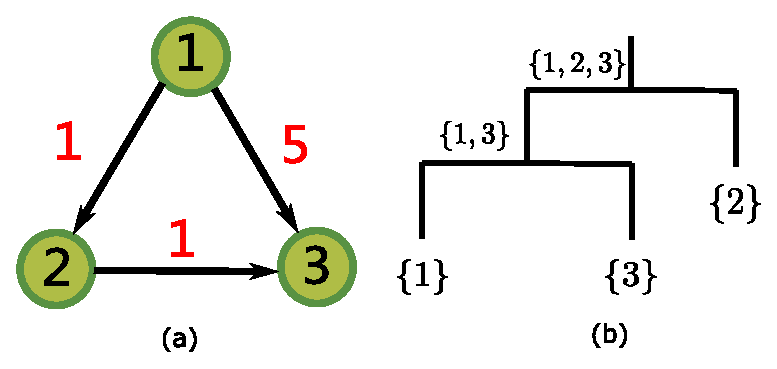
\includegraphics[width=0.44\textwidth]{pic/example_directed.eps}
	\end{center}
	\caption{An illustration of info-clustering and its corresponding clustering tree}\label{fig:first_illustration}
\end{wrapfigure}

For sufficiently large $\gamma$, $C_{\gamma} (Z_V)$ will become empty set. The largest threshold value which makes such transition is denoted by $\gamma_N$, which has the following expression:
\begin{equation}\label{eq:gammaN}
\gamma_N = \max_{A\subseteq V, \abs{A}>1} I(Z_A)
\end{equation}
Suppose $\gamma_N=I(Z_B)$ and $B$ is the maximal set to achieve the maximum. This convention is used in the following sections.

\begin{example}
	Consider a graph $G(V,E)$ with $V=\{1,2,3\}, E=\{(1,2),(2,3),(1,3)\}$. The weight values are $w_{12}=1, w_{13}=5, w_{23}=1$. The graph is shown on Fig.\ref{fig:first_illustration}.(a). Let $\P_2 = \{\{1,3\},\{2\}\}$, then $f[\P_2] = 2 $ and $I_{\P_2}(Z_V) = 2$ from equation \eqref{eq:IP}. Let $\P_3 = \{\{1\},\{2\},\{3\}\}$, then $f[\P_3] = 7$ and $I_{\P_3}(Z_V)=3.5$. Therefore $I(Z_V) = \min\{I_{\P_2}(Z_V), I_{\P_3}(Z_V), \dots\} = 2$. 
	\begin{equation*}
	C_{\gamma}(Z_V)	=\begin{cases}
					\{\{1,2,3\}\} & \gamma < 2 \\
					\{\{1,3\}\} & 2\leq \gamma < 5 \\
					\emptyset & \gamma \geq \gamma_N = 5
		\end{cases}
	\end{equation*}
	The clustering tree $\mathcal{T}$ for this example consists of $\{1,2,3\}$ as root, $\{1,3\}$ as stem and $\{1\},\{2\},\{3\}$ as leaves, which are shown on Fig.\ref{fig:first_illustration}.(b).
\end{example}	

\subsection{Info-Detection Method}
For our Info-Detection proposal, we use $\gamma_N$ as a threshold to detect anomaly.  Given $G(V, E)$, we first compute $\gamma_N$ and $B$. Then nodes in $B$ are inliers while nodes in $V\backslash B$  are outliers. We can score outlier $Z_j$ for $j \in V\backslash B$ with the depth of the set $\{j\}$ in the hierarchical tree. Below is a simple example showing how Info-Detection is used.
\begin{example}
	\begin{figure}[!ht]
		\centering
		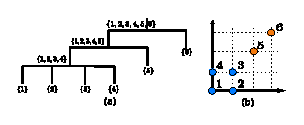
\includegraphics[width=9cm]{pic/outlier_example.eps}
		\caption{Info-Detection applied to 6 points on Cartesian plane}\label{fig:ex}
	\end{figure}
	Consider a graph consisting of 6 nodes. Each node is corresponding to a point on Cartesian plane (Fig. \ref{fig:ex}.(b)). The grid has one unit and the edge weight $w_{ij} = \exp(-d_{ij}^2)$ where $d_{ij}$ is the Euclidean distance between $x_i$ and $x_j$ on the plane. For example, $w_{45} = \exp(-5)$. The edge direction is from $i$ to $j$ for $i<j$. From equation \eqref{eq:gammaN}, we can compute $B=\{1,2,3,4\}$ and $\gamma_N = \frac{4\exp(-1)+2\exp(-2)}{3}\approx 0.58$. The whole hierarchical tree $\mathcal{T}$ can also be computed, which is shown on Fig. \ref{fig:ex}.(a). The outlier score for $Z_6$ is higher than $Z_5$ from the tree depth interpretation.
\end{example}


For newly added node $i'$. Let $V'=B\cup \{i'\}$, we can compute $\gamma'_N$ for $G(V', E(V'))$ and compare it with $\gamma_N$. If $\gamma'_N>\gamma_N$, $i'$ is normal observation since it is more integrated with existing nodes. Otherwise, $i'$ is an anomaly. It can be shown that we do not need to compute $\gamma'_N$ to determine whether $\gamma'_N>\gamma_N$. We summarize our main result as follows:
\begin{proposition}\label{prop:main}
\begin{equation}
\gamma'_N > \gamma_N \iff  \sum_{i \in B} w_{ii'} > \gamma_N 
\end{equation}
\end{proposition}
From Proposition \ref{prop:main}, we can see that the computational overhead to check whether new data is normal is linear to the size of existing normal data. 

Info-Detection requires $\gamma_N$ and $B$, whose computation is not a trivial task and is the main focus of the next Section.

\section{Improved Principal Sequence of Partition}\label{sec:Alg}
\subsection{Existing Algorithms}
It has been found that the mathematical structure of info-clustering is the same with that of principal sequence of partition (PSP) of graph. Let $\P_1, \dots, \P_k$ denote PSP sequence where $\P_1 = \{V\}, \P_{i+1} \preceq \P_i$ and $\P_k = \{\{1\},\dots,\{k\}\}$.
Each $\P_i$ is the solution to the following optimization problem:
\begin{align}
h_{\P}(\lambda) &=  f[\P] - \abs{\P} \lambda  \label{eq:hPL}\\
h(\lambda) &= \min_{\P \in \Pi'(V)} h_{\P}(\lambda) \label{eq:hlambda}
\end{align}
We call $\lambda^*$ a critical value for PSP if $\P_i, \P_{i+1}$ are both minimizer for $h(\lambda^*)$ in \eqref{eq:hlambda}.
The largest critical value is equal to $\gamma_N$ and the largest set in $\P_{k-1}$ is equal to $B$. 

Info-clustering is originally implemented by solving equation \eqref{eq:hlambda} for different critical values \cite{RN3}. For given critical value, a procedure called Dilworth truncation (DT) can be used to get the minimum value and corresponding partition for \eqref{eq:hlambda}. The implementation in \cite{RN3} has $\abs{V}^2 \textrm{MF}(G)$ time complexity while \textrm{MF} represents the time complexity of maximum flow algorithm for a graph $G$. 

An improvement is proposed in \cite{RN4} using parametric maximum flow to finish the job. Although this method can achieve $\abs{V} \textrm{MF}(G)$ time complexity theoretically, in practice it performs not well. Besides, it also increases the space complexity and has the floating point accuracy problem. 

\subsection{Improved Algorithm} 
In this section, we give an improvement which achieves $\abs{V} \textrm{MF}(G)$ time complexity in general, and the space complexity is the same with \cite{RN4}. Specifically,
we notice that different invocation of Dilworth truncation is independent and does not utilize the intrinsic hierarchical structure in the original version of PSP algorithm \cite{RN3}. If the hierarchical tree structure is used, we can invoke Dilworth truncation (DT) on smaller graph in later computation and make the total computation one order of magnitude faster than previous.

To be more specific, suppose we get $P_i = {C_1, \dots, C_t}$ for the first invocation of DT. Then we can compute PSP for each $C_i(i=1,\dots, t)$ respectively and construct those $P_j(j>i)$ from the subgraph computation. For $P_j(j<i)$, we can contract the graph $G$  to $G^t$ which has $t$ nodes by contracting each $C_i$ to a single node. By applying DT to $G^t$ can we get $P_j(j<i)$. We summarize our improved version in Algorithm \ref{alg:psp_i_simplified}.

\begin{algorithm}
	\caption{An Improved Principal Sequence of Partition Algorithm}\label{alg:psp_i_simplified}
	\begin{algorithmic}[1]
		\REQUIRE a directed graph $G(V, E)$; edge weight map $c(e)$ for $e\in E$
		\ENSURE a hierarchical tree $\mathcal{T}(K, E)$ where $K \subseteq 2^{V}$ is node set and $E$ is edge set.
		\STATE initialize tree $\mathcal{T}$ with $V$ as root node, $\{j\}(j\leq \abs{V})$ as leaf node and no stem node.
		\STATE \texttt{Split}($G, V$)
		\FUNCTION{\texttt{Split}($\widetilde{G}, \widetilde{V}$)}
		\STATE $w$ is the summation of all edge weights of $\widetilde{G}$ 
		\STATE $\gamma' = \frac{w}{\abs{V(\widetilde{G})}-1}$ where $V(\widetilde{G})$ is the node set of graph $\widetilde{G}$ \label{alg:gamma_apostrophe}
		\STATE $(\tilde{h}, P') = \texttt{DT}(\widetilde{G}, \gamma')$ where $\P'$ is minimizer of $h(\gamma')$ in equation \eqref{eq:hlambda} and $\tilde{h}$ is the corresponding minimum value.  \label{alg:DT}
		\IF{$\tilde{h} = - \gamma'$}
		\STATE add edge weight $\gamma'$ in $\mathcal{T}$ starting from $\widetilde{V}$ to its children
		\ELSE
		\FOR{$S$ in $P'$ and $\abs{S}>1$}
		\STATE make each children of $\widetilde{V}$ in $\mathcal{T}$ have new parent $S$		
		\STATE make the parent of $S$ be $\widetilde{V}$
		\STATE \texttt{Split}($\widetilde{G}[S], S$) where $\widetilde{G}[S]$ is the subgraph of $\widetilde{G}$ restricted on $S$
		\STATE contract $S$ to a single node in $\widetilde{G}$ % graph \widetilde{G} is modified
		\ENDFOR 
		\STATE \texttt{Split}($\widetilde{G}, \widetilde{V}$)		
		\ENDIF
		\ENDFUNCTION
	\end{algorithmic}
\end{algorithm}
	
%	It is shown in \cite{RN8} that $\gamma_N$ has an alternative form
	
%	\begin{equation}\label{eq:gammaN_alternative}
%	\gamma_N = \max_{A \subseteq V, \abs{A}>1} \frac{\sum_{(i,j)\in E(A)} w_{ij}}{\abs{A}-1}
%	\end{equation}
	
\begin{figure}[!ht]
	\centering
	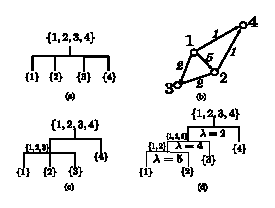
\includegraphics[width=10cm]{pic/alg_illustration.eps}
	\caption{Improved PSP for graph in (a), hierarchical tree evolves from (b), (c) to (d) }\label{fig:alg_eg}
\end{figure}

\begin{example}
	We use a simple example to explain Algorithm \ref{alg:psp_i_simplified}. Consider a graph $G(V, E)$ with $V=\{1,2,3,4\}, E=\{(1,2),(1,3),(2,3),(1,4),(2,4)\}$. The weight values are $w_{13}=2, w_{12}=5, w_{23}=2, w_{14}=1, w_{24}=1$. The graph is illustrated
	in Fig. \ref{fig:alg_eg} (a). Initially, the hierarchical tree is shown in Fig. \ref{fig:alg_eg} (b). Computing $\gamma' = \frac{11}{4-1}, \tilde{h} = -\frac{16}{3} < -\gamma' $ and $\P' = \{\{1,2,3\},\{4\}\}$ from line \ref {alg:DT} in Algorithm \ref{alg:psp_i_simplified} we get the hierarchical tree shown in Fig. \ref{fig:alg_eg} (c).
	
	Then we run PSP for the subgraph $G[\{1,2,3\}]$, $\gamma' = \frac{9}{2}, \tilde{h} = -5 < -\gamma'$ and $\P= \{\{1,2\},\{3\}\}$ we get the tree shown in Fig. \ref{fig:alg_eg} (d). The other computation gives the edge weight of $\mathcal{T}$ shown in Fig. \ref{fig:alg_eg} (d).
\end{example}		

To analyze the time complexity of Algorithm \ref{alg:psp_i_simplified}. We suppose $\abs{V} = n, \abs{E} = O(n^2)$ and highest-relabel preflow algorithm is used to solve the maximum flow problem. Then \texttt{DT} routine has $O(n^4)$ time complexity. 
We use $T(n)$ to represent the time complexity of \texttt{Split} when the graph has $n$ nodes. Under very general conditions, we can show that $T(n) = O(n^4)$. 

In Algorithm \ref{alg:psp_i_simplified}, the graph contraction is done on the input graph without creating extra structures. The space complexity is the same with the storage needed for the input graph. 

Our improvement is not restricted to Info-Detection scenario. It can be used in general graph partition problems when PSP structure is needed.

\section{Experimental Results}\label{sec:Experiemt}
In this Section, we first illustrate the decision boundary of Info-Detection by two artificial datasets. Then we compare the running time of our implementation of PSP with previous work. Finally we conduct an experiment matrix, in which Info-Detection is compared with other commonly used outlier detection algorithms on both artificial and real-world datasets.

Info-Detection uses the boundary curve to make prediction on new observations and the boundary curve has the following form from Proposition \ref{prop:main}:
\begin{equation}
\sum_{j \in B} \exp(-\gamma \norm{x - x_j}^2)= \gamma_N
\end{equation}
The weight is chosen by Gaussian kernel, which produces reasonable good result for these two artificial datasets. As shown by Fig. \ref{fig:boundary}. (a) and (b), the boundary curve for Info-Detection is approximately the closure of the set of inliers. We also draw the decision boundary for the elliptic envelope method in Fig. \ref{fig:boundary}.(c). Since the latter method assumes the inlier data is distributed in convex region, the decision boundary is an ellipse, which is not the ground truth.
\begin{figure}[!ht]
	\centering
	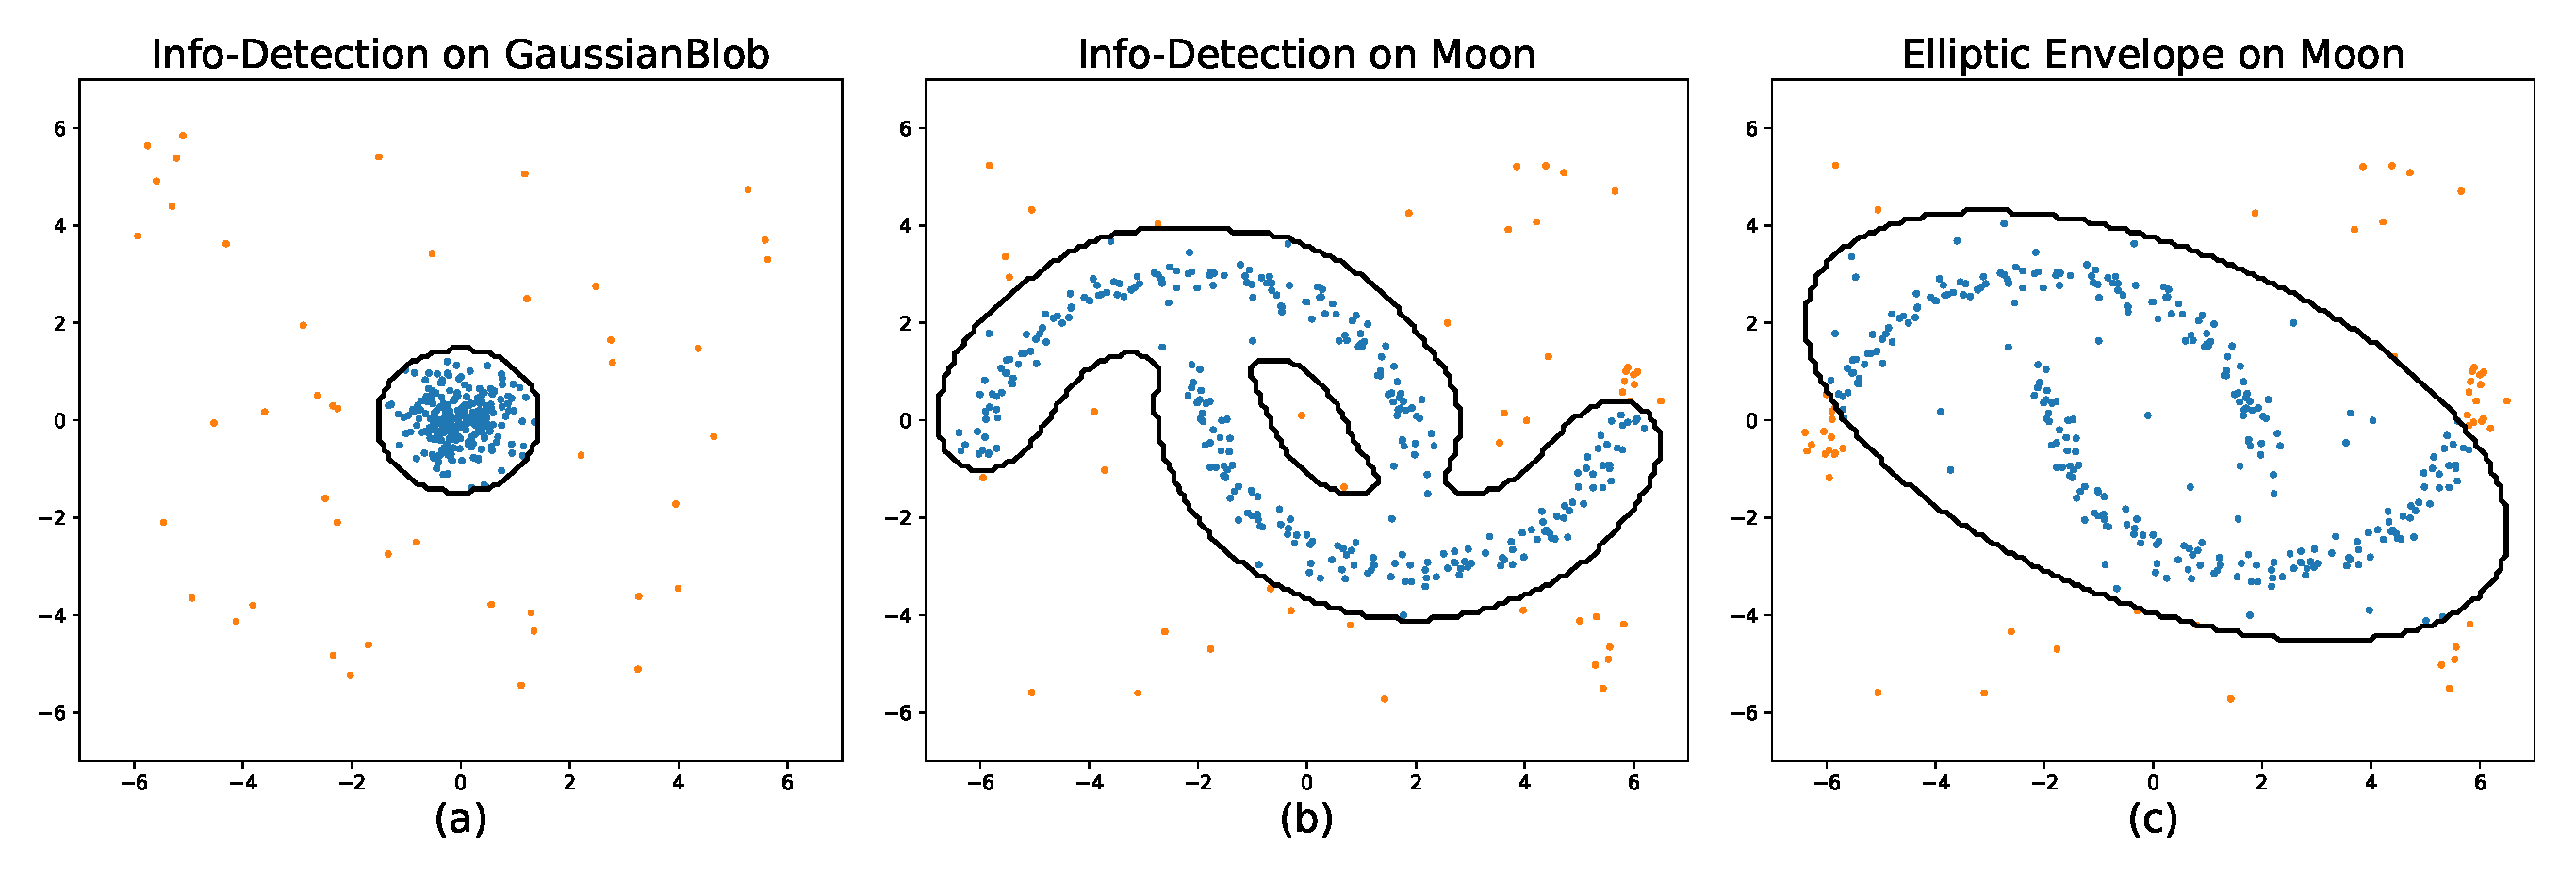
\includegraphics[width=\textwidth]{pic/outlier_boundary_illustration.eps}
	\caption{Detection boundary lines of different methods on different artificial dataset}	\label{fig:boundary}
\end{figure}

Next we compare our implementation of PSP with previous methods \cite{RN3,RN4}. The comparison is done on Gaussian blobs dataset ($\abs{E}=O(\abs{V}^2)$) and a graph dataset with two hierarchical levels($\abs{E}=O(\abs{V}^{3/2})$). We use the CPU times to measure the practical speed of each implementation and the result in Fig.\ref{fig:er}.(a,b) shows our implementation is much faster than previous ones.

\begin{figure}[!ht]
\centering
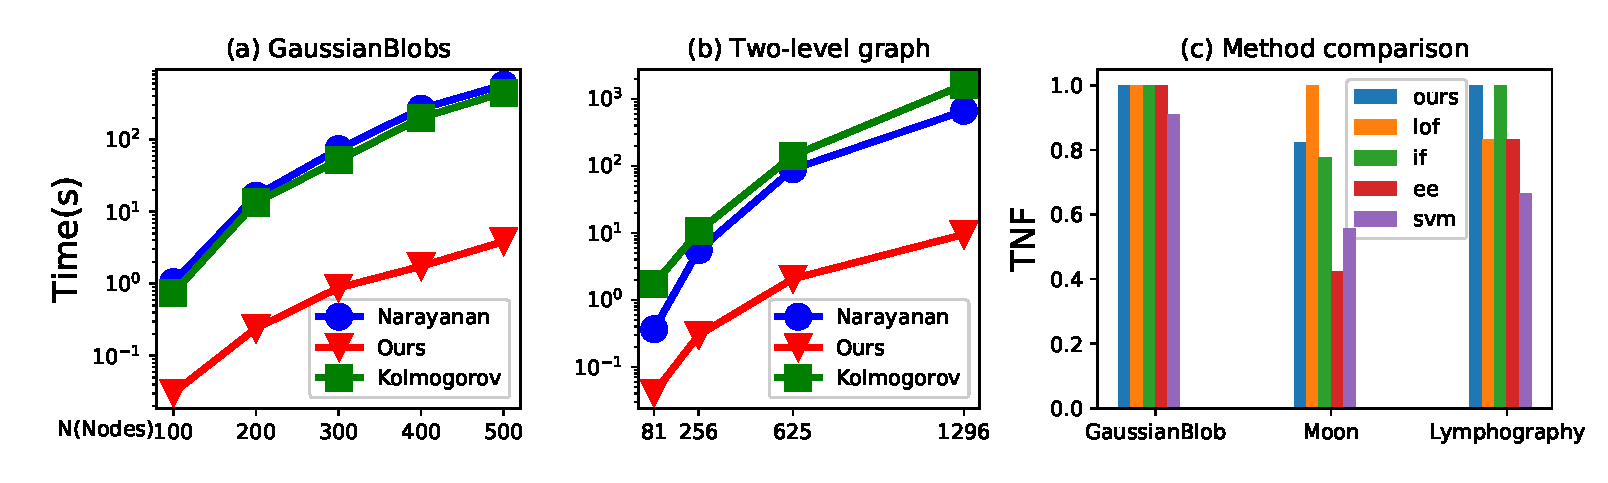
\includegraphics[width=\textwidth]{pic/experimental_results_triple.eps}
\caption{Experimental results on datasets}\label{fig:er}
\end{figure}

We also compare Info-Detection with other commonly used techniques on three dataset: GaussianBlob, Moon and UCI Lymphography. The other methods include local outlier factor \cite{Breunig}, isolation forest \cite{if}, elliptic envelope \cite{rousseeuw1999fast} and one class SVM \cite{svm}. We use two metrics to measure the overall performance of the detection: true positive rate (TPR) and true negative rate (TNR). The inlier is treated as positive sample. TPR measures the percentage of right detection in inlier set while TNR measures that in outlier set. It is difficult for a method to achieve high score on both two metrics. We manage to maximize TNR while controlling TPR $\geq 90\%$ for each method. The result for TNR in Fig.\ref{fig:er}.(c) shows that Info-Detection is competitive with local outlier factor and outperforms other methods on these datasets.

\section{Conclusion}\label{sec:Conclusion}
In this paper, we propose Info-Detection, which is a cluster-analysis based method and does not require the number of outliers in advance. We design an efficient algorithm for Info-Detection based on existing PSP algorithms. By experiments we show that Info-Detection outperforms other methods.  
\section*{Acknowledgment}

The research of Shao-Lun Huang was funded by the Natural Science Foundation of China 61807021, Shenzhen Science and Technology Research and Development Funds (JCYJ20170818094022586), and Innovation and entrepreneurship project for overseas high-level talents of Shenzhen (KQJSCX20180327144037831).
%
% ---- Bibliography ----
%
% BibTeX users should specify bibliography style 'splncs04'.
% References will then be sorted and formatted in the correct style.
%
\bibliographystyle{splncs04}
\bibliography{exportlist}
%


\end{document}
